\section{A recovery backstop for interbank contagion}
\label{sec:contingent_support}\label{sec:interbank-recovery-backstop}

Section~\ref{sec:ex-post-compensation} guarantees repayments relative to the original preferred equilibrium. We now consider protection defined directly from losses at settlement: the facility covers a fraction of the repayment capacity destroyed by bank default costs. We ask the same two questions: does this rule eliminate adverse equilibria, and what financial resources does it require? Timing and external financing are unchanged.

\subsection{The recovery-backstop rule and clearing}\label{subsec:interbank_recovery_backstop}

Let $\eta\in[0,1]$ be the fraction of default-cost losses covered. For a defaulting bank $j$, ordinary repayment is $R_j=\lambda_j^BA_j/D_j$. Its bank creditors receive
\begin{equation}
 \widehat R_j(s;\eta)=\min\left\{1,
 R_j+\eta\left[A_j/D_j-R_j\right]\right\}.
 \label{eq:interbank_backstop_repayment}
\end{equation}
For a nondefaulting bank, $\widehat R_j=1$; nonbank creditors receive ordinary repayment. The cap prevents overpayment when prudential distress occurs with positive pre-cost equity. At full coverage, bank creditors receive pre-cost repayment capacity capped at par; any fundamental asset shortfall remains uncovered.


Bank resources use guaranteed receipts on interbank claims:
\begin{equation}
 A_i(s)=a_i(s)+\sum_{j\in\mathcal B}x_{ij}\widehat R_j(s;\eta).
 \label{eq:interbank_backstop_assets}
\end{equation}
Together with \eqref{eq:bank_repayment}, this determines bank defaults and repayments jointly. As with the repayment floor, protection changes creditor banks' receipts and therefore their own repayment capacity. Here the protection is tied to the debtor's default-cost loss, rather than to a preferred-equilibrium target.

\subsection{Effects on banking equilibria}

We solve the policy clearing system for all sixteen sovereign states, varying common coverage from 0\% to 100\% in five-percentage-point steps. Multiplicity falls from eight states without intervention to six at 25\% coverage, two at 30\% and one at 35\%. At 40\% and every higher tested coverage, all states have a unique banking equilibrium (Figure~\ref{fig:interbank_recovery_backstop_grid}, panel a).\footnote{At each coverage we enumerate all banking equilibria using the solver in Appendix~\ref{app:solver_details}. A finer sweep in one-percentage-point steps first finds uniqueness in all states at 36\%. These sweeps identify sufficient coverage levels, rather than a minimum over continuous coverage as characterized for the repayment floor in Section~\ref{sec:minimum-floor-budget}.}

The backstop therefore also removes multiplicity in this calibration. It does not generally deliver full repayment: fundamental Italian and Spanish bank credit events can persist. These equilibrium results are obtained state by state and require no probabilities over sovereign states or weights over banking equilibria.

\subsection{Payments required by the backstop}

For policy equilibrium $e$ in state $s$, let $R_j^e(s)$ denote ordinary repayment and $\widehat R_j^e(s;\eta)$ the protected rate. The facility pays
\begin{equation}
 K(e,s;\eta)=\sum_jL_j^{BB}[\widehat R_j^e(s;\eta)-R_j^e(s)]_+.
 \label{eq:interbank_backstop_cost}
\end{equation}
To assess the largest payment requirement, we maximize $K(e,s;\eta)$ over all policy equilibria and sovereign states, as in the compensation benchmark of Section~\ref{sec:ex-post-compensation}. Panel b of Figure~\ref{fig:interbank_recovery_backstop_grid} reports this maximum as a percentage of aggregate bank debt. It requires no probability or equilibrium-selection weights.

At 40\% coverage, the largest payment is EUR~19.3 billion, or 0.09\% of bank debt. At the round half-coverage benchmark it is EUR~24.2 billion, or 0.12\%. Unlike the repayment floor at its target, the recovery backstop can make payments in the surviving equilibrium because it protects creditors against default-cost losses that remain after multiplicity has been eliminated. These amounts are disbursements under the recovery rule; Section~\ref{sec:minimum-floor-budget}'s EUR~60.6 billion is backing for a different promise, which makes no equilibrium transfers.

Panel b is non-monotone because higher coverage both increases reimbursement for continuing bank defaults and can eliminate costly default equilibria. At 35\% coverage, the maximum payment is about EUR~67 billion in the all-sovereign-default state, in an adverse equilibrium that includes French bank default. At 40\%, that equilibrium has disappeared; the maximum shifts to the Italian-and-Spanish sovereign-default state and falls to EUR~19.3 billion. Payments then rise with coverage of the remaining defaults, until the cap on creditor receipts binds.

Appendix~\ref{app:ocr_robustness} reports average losses and payments conditional on a sovereign crisis, together with their sensitivity to sovereign dependence and equilibrium-selection weights. Those averages summarize the distribution of outcomes; they are not used to establish the equilibrium effects or maximum payment requirements above.

\begin{figure}[tp]
\centering
\floatcaption{Equilibrium effects and maximum payments of the common recovery backstop}{Coverage varies in five-percentage-point steps. Panel (a) counts sovereign states with multiple banking equilibria. Panel (b) gives the largest facility payment across all sovereign states and policy equilibria, as a percentage of aggregate clearing debt. Both panels are independent of sovereign probabilities and equilibrium-selection weights. Creditor receipts are capped at par.}
\label{fig:interbank_recovery_backstop_grid}

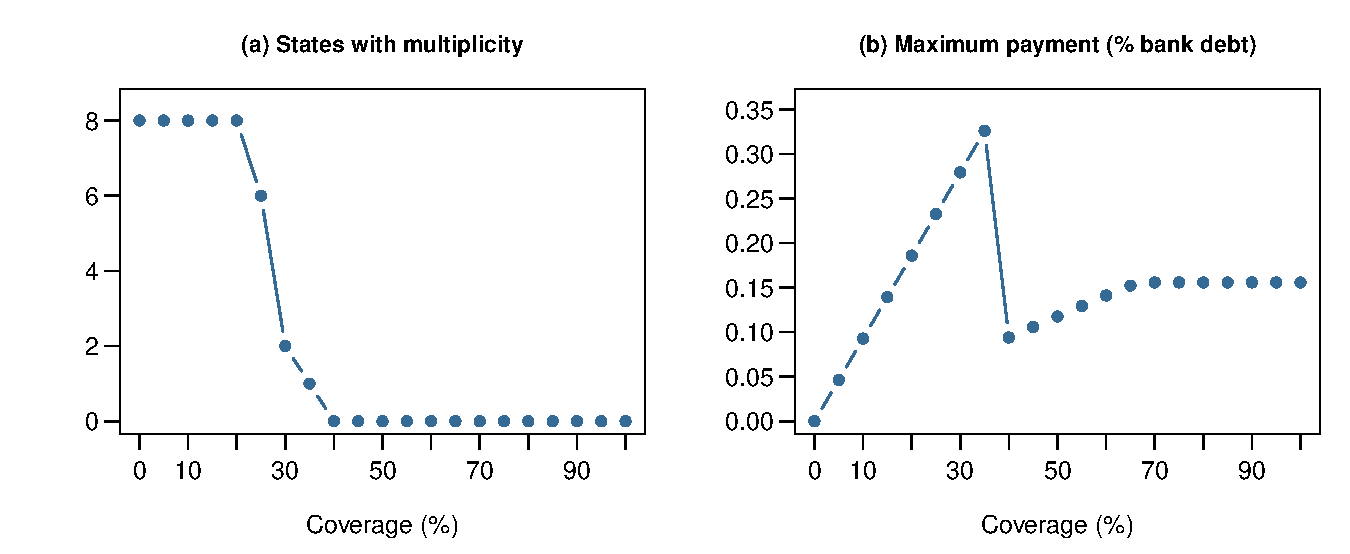
\includegraphics[width=\linewidth]{Figures/interbank_recovery_backstop_grid.pdf}

\end{figure}

\FloatBarrier
